\documentclass[titlepage]{scrartcl}
\usepackage{enumitem}
\usepackage[british]{babel}
\usepackage[style=apa, backend=biber]{biblatex}
\DeclareLanguageMapping{british}{british-apa}
\usepackage{url}
\usepackage{float}
\usepackage[labelformat=empty]{caption}
\restylefloat{table}
\usepackage{perpage}
\MakePerPage{footnote}
\usepackage{abstract}
\usepackage{graphicx}
% Create hyperlinks in bibliography
\usepackage{hyperref}
\usepackage{amsmath}

\usepackage[T1]{fontenc}
\usepackage[utf8]{inputenc}
\usepackage{blindtext}
\setkomafont{disposition}{\normalfont\bfseries}

\graphicspath{
    {./resources/},
}
\addbibresource{~/Documents/library.bib}

\newsavebox{\abstractbox}
\renewenvironment{abstract}
  {\begin{lrbox}{0}\begin{minipage}{\textwidth}
   \begin{center}\normalfont\sectfont\abstractname\end{center}\quotation}
  {\endquotation\end{minipage}\end{lrbox}%
   \global\setbox\abstractbox=\box0 }

\usepackage{etoolbox}
\makeatletter
\expandafter\patchcmd\csname\string\maketitle\endcsname
  {\vskip\z@\@plus3fill}
  {\vskip\z@\@plus2fill\box\abstractbox\vskip\z@\@plus1fill}
  {}{}
\makeatother

\DeclareCiteCommand{\citeyearpar}
    {}
    {\mkbibparens{\bibhyperref{\printdate}}}
    {\multicitedelim}
    {}

% MATLAB Code block stuff...
\usepackage{color}
\usepackage{listings}

\definecolor{dkgreen}{rgb}{0,0.6,0}
\definecolor{gray}{rgb}{0.5,0.5,0.5}

\lstset{language=Matlab,
   keywords={break,case,catch,continue,else,elseif,end,for,function,
      global,if,otherwise,persistent,return,switch,try,while},
   basicstyle=\ttfamily,
   keywordstyle=\color{blue},
   commentstyle=\color{gray},
   stringstyle=\color{dkgreen},
   numbers=left,
   numberstyle=\tiny\color{gray},
   stepnumber=1,
   numbersep=10pt,
   backgroundcolor=\color{white},
   tabsize=4,
   showspaces=false,
   showstringspaces=false}

\begin{document}
    \title{ECS707P Fundamentals of DSP}
    \subtitle{\LARGE{Lab 1 Report}}
    \author{Sam Perry - ec16039}

    \maketitle

    \section*{Section 2.1 Buoy data parsing function}
    \begin{lstlisting}
% Declare a function that takes a signle argument (the
% file path) and returns a 'data' object containing the
% data parsed from the file object.  A count integer is
% also returned with the number of entries read from
% file.
function [data, count] = readbuoydata(datafile)

    % Create a file object with the path provided by the
    % 'datafile' variable
    fid = fopen(datafile,'r');
    % Read first two header lines of file so that they
    % are ignored in processing below.
    tline = fgetl(fid);
    tline = fgetl(fid);

    % Parse each line of the file from line 3 onwards
    % and store in variable 'A' first argument specifies
    % the file object.
    % second arguments specifies the data type to expect
    % for each of the 10 elements per line.
    % the third argument specifies to read 10 elements
    % per line, and to read until the end of the file.
    [A,count] = fscanf(fid, ...
    '%d %d %d %d %d %f %f %d %f %f',[10 inf]);

    % Creates a member of the data object that contains
    % dates in the 'serial date number' format
    data.date = datenum([A(1:5,:); zeros(1,size(A,2))]')';
    data.Hs = A(6,:); % significant wave height
    data.Tp = A(7,:); % peak period
    data.Dp = A(8,:); % peak period direction
    data.Ta = A(9,:); % average period
    data.SST = A(10,:); % sea surface temperature

    % Close the file 
    fclose(fid);
    \end{lstlisting}

    \section*{Section 2.2 Peak Period and Wave Height Plots}

    \begin{figure}[H]
        \makebox[\textwidth]{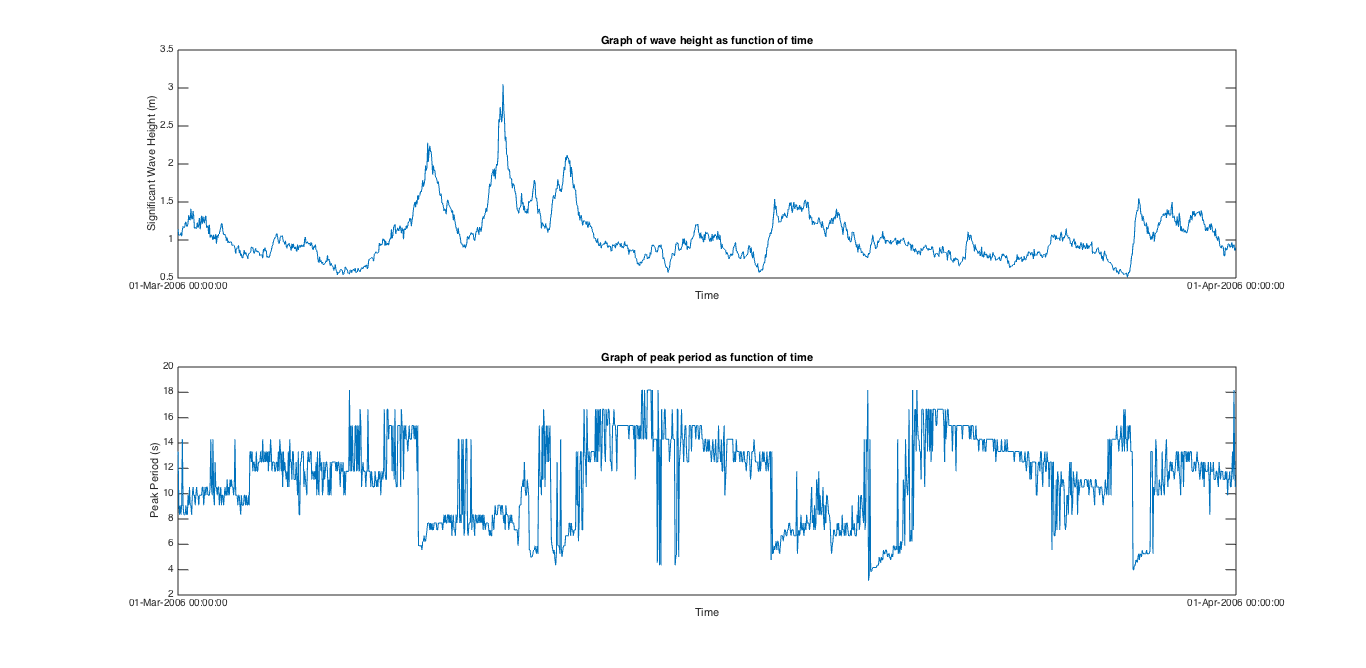
\includegraphics[width=1.3\textwidth]{HeightPeriodPlot}}
    \end{figure}

    \section*{Section 2.3 Moving Average Filter Function}
    \begin{lstlisting}
% Function takes an 1-dimensional input signal and
% an M value (>0) 
% A filtered signal of the same size is returned
function [outputSignal] = movingAverage(inputSignal, M)
    % Initialize output array with zeros.
    outputSignal = zeros(1, length(inputSignal));
    % Pad input with zeros at the begining.
    inputSignal = [zeros(1, M-1), inputSignal];

    % For each sample in input...
    for n = M:length(inputSignal)
        % Take the last M samples and save their
        % mean value as the output sample.
        outputSignal(n-M+1) = mean(inputSignal(n-M+1:n));
    end
    \end{lstlisting}

    \section*{Section 2.4 Filtered Peak Period Data Plots}
    \begin{figure}[H]
        \makebox[\textwidth]{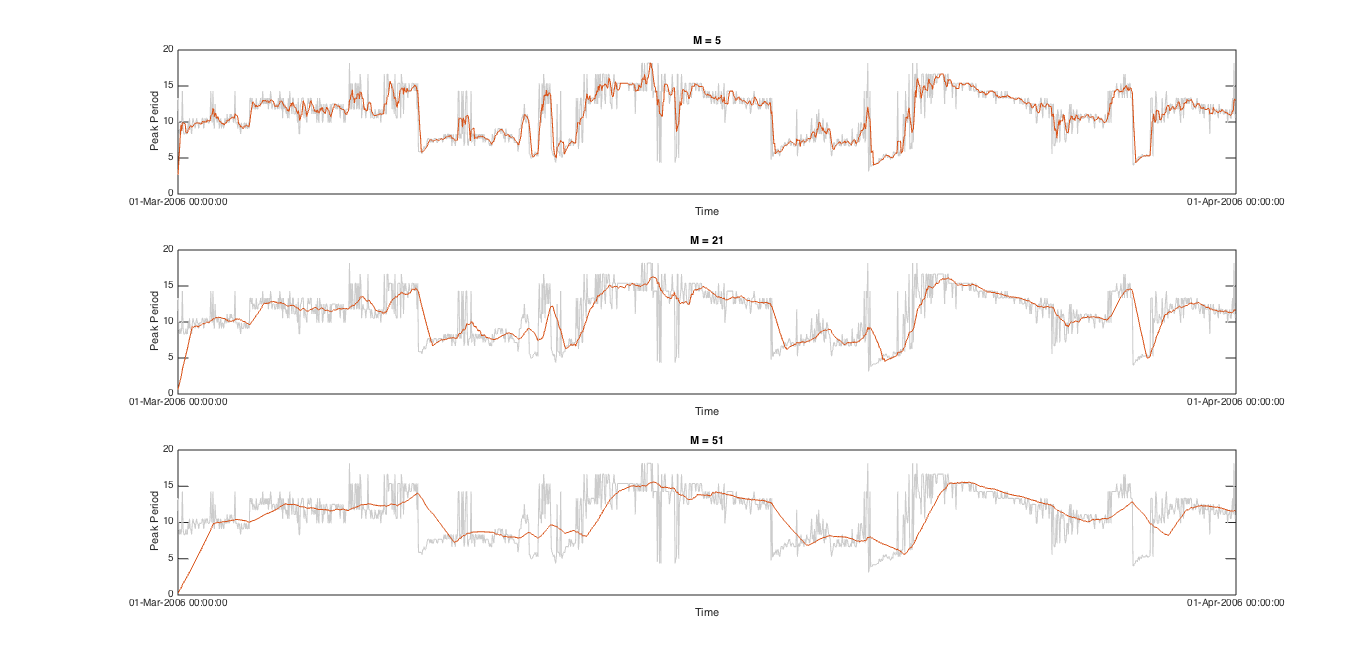
\includegraphics[width=1.3\textwidth]{MovingAveragePlot}}
    \end{figure}

    \section*{Section 2.5 Questions}
    \subsection*{Q1. What do you observe as $M$ increases?}
    The output signal appears to be smoothed at increasing amounts as values
    for $M$ increase.

    \subsection*{Q2. Why do you think you observe this ``thing''?}
    Increasing $M$ increases the size of the window of signal averaged to
    form each samples in the output signal. By averaging larger windows of
    signal to form the output, output samples will deviate less from the
    previous sample due to the increased similarity between the consecutive
    windows. This causes the smoothing effect observed.

    \subsection*{Q3. What is happening at the beginning of the averaged dataset, and why does it happen?}
    There is a ramp up from 0 that is increasingly prominent with increasing
    values of $M$. This is due to the $M-1$ zeros padding the start of the
    input signal to allow initial samples to be processed. As these are
    included in the averaging of input samples, they decrease the value of
    output samples. As $n$ increases, less zero-padding is included in the
    average, causing a ramp up. As there are more zeros with larger values of
    $M$, this effect is more prominent with higher values of $M$ as it will
    affect $M-1$ samples at the beginning of the output signal.

    \subsection*{Q4. What happens to the running average when the peak period suddenly drops?}
    If the peak period suddenly drops and remains stable at the new value, then
    the running average will drop to this value in $M$ samples. Essentially the
    running average will reach any new value in $M$ samples if that new value
    remains constant, if it doesn't then the running average will vary based on
    the average of samples in the consecutive windows. For this reason, large
    windows filter out quick drops or spikes in the input, as the mean of the
    window is still relatively close to the majority of samples.

    \subsection*{Q5. Are these drops preserved?}
    Sudden drops will be smoothed increasingly into ramps with larger values of
    $M$ for the reasons stated above.

    \subsection*{Q6. Are the wave trains more clear?}
    Wave trains are clearer with higher values of $M$.  Due to the removal of
    small fluctuations in the signal, the overall contour of the averaged
    signal shows the increase and gradual decrease more clearly.

    \section*{Section 2.6 Filtered Wave Height Plots}
    \begin{figure}[H]
        \makebox[\textwidth]{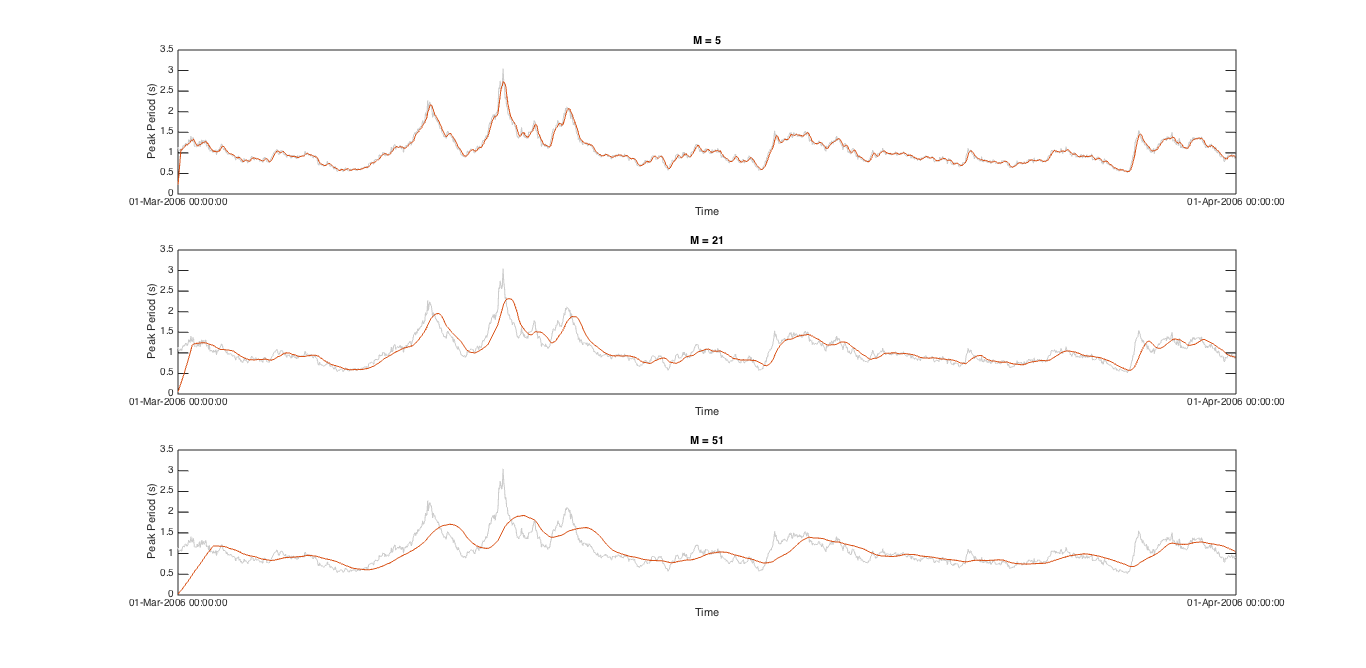
\includegraphics[width=1.3\textwidth]{MovingAverageWavePlot}}
    \end{figure}

    \section*{Section 2.7 Questions}
    \subsection*{Q1. Do you observe anything different in the plots from 2.6 to those you saw in 2.4?}
    Aside from the time shift mentioned in the lab instructions, a significant
    observation is that for wave height, lower values of $M$ resemble the
    original signal more closely than the equivalent plots of peak period. As
    there are fewer abrupt fluctuations in the original signal, the output at
    $M=5$ is very similar to the input. This is not true of the peak period as
    the original signal has many small variations that are smoothed even with
    small values.

    \subsection*{Q2. How does the size of this shift relate to M?}
    The samples will lag by $M\div2$ samples. (Explained below...)

    \subsection*{Q3. Explain why the peaks move? (in complete sentences)}
    This lag is caused by the window comprising entirely of samples on one side
    of $n$. As the window centres around samples before $n$, the output sample
    will be an average of samples around the centre of the window rather than
    centring on $n$. This causes the lag of half a window size.

    \section*{2.8 Non-causal moving average filter}

    %\subsection*{}
    \begin{figure}[H]
        \caption{Peak Period Plots}
        \makebox[\textwidth]{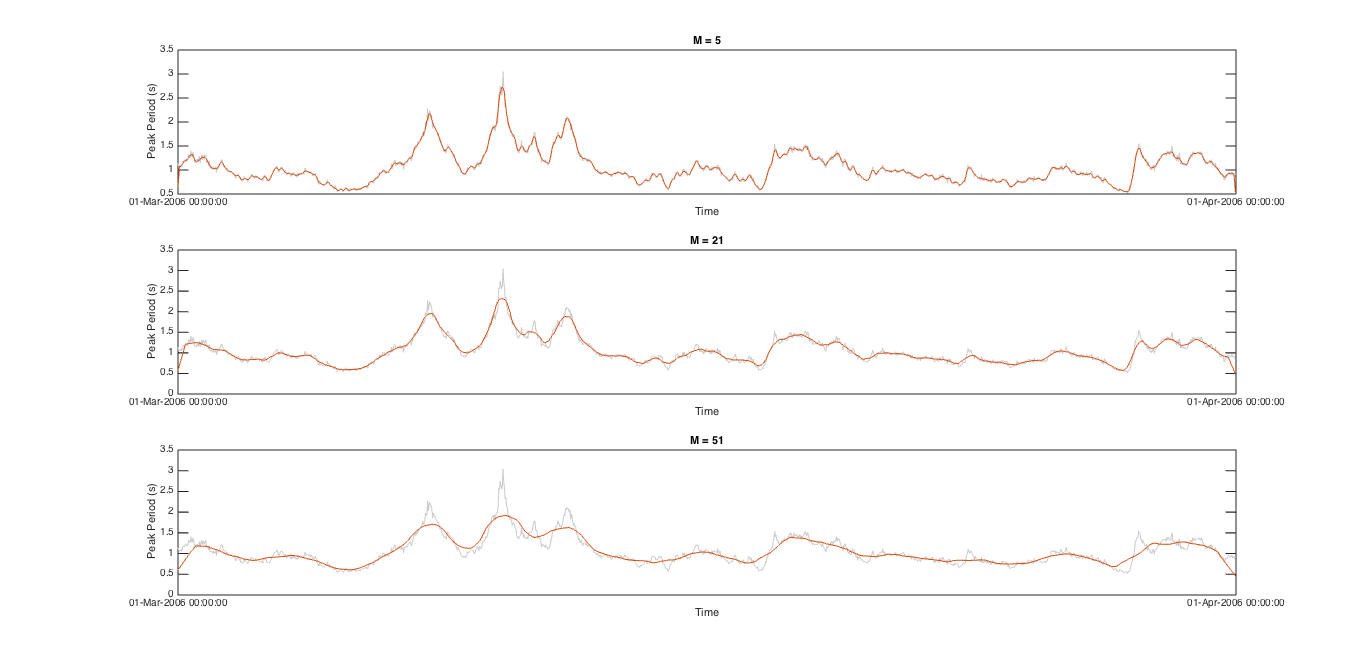
\includegraphics[width=1.3\textwidth]{NCMovingAveragePeakPlot}}
    \end{figure}
    
    %\subsection*{}
    \begin{figure}[H]
        \caption{Wave Height Plots}
        \makebox[\textwidth]{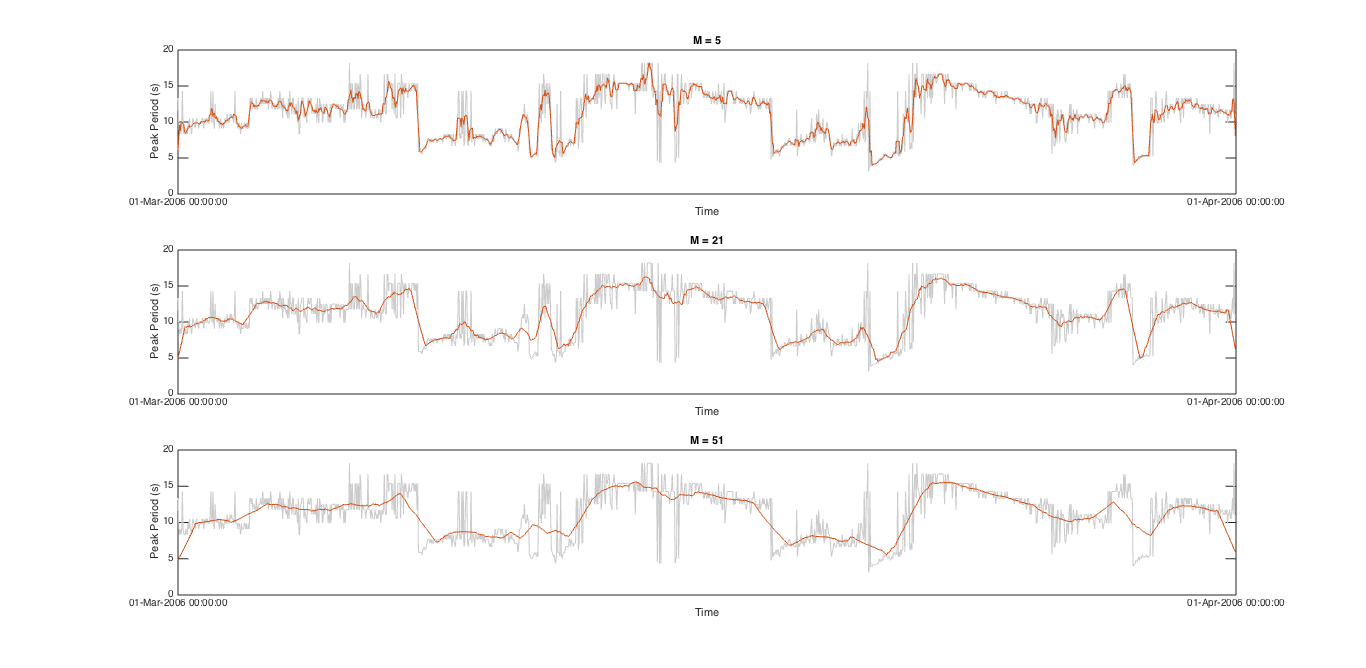
\includegraphics[width=1.3\textwidth]{NCMovingAverageWavePlot}}
    \end{figure}

    \subsection*{Non-causal moving average filter code}
    \begin{lstlisting}
% Function takes an 1-dimensional input signal and
% an even M value (>0) 
% A filtered signal of the same size is returned
function [outputSignal] = nonCausalMovingAverage(inputSignal, M)
    % Check that M is odd
    validateattributes(1, {'numeric'}, {'odd'});

    % Initialize output array with zeros.
    outputSignal = zeros(1, length(inputSignal));
    % Pad input with zeros at beginning and end
    inputSignal = [zeros(1, (M-1)/2), inputSignal, ...
        zeros(1, (M-1)/2)];

    % For each sample in input...
    for n = M:length(inputSignal)
        % Take the last M samples and save their
        % mean value as the output sample.
        outputSignal(n-M+1) = mean(inputSignal(n-M+1:n));
    end
    \end{lstlisting}


    % \printbibliography
\end{document}
